\documentclass[]{article}
\usepackage{fullpage, setspace, listings, color, subcaption, graphicx}
\graphicspath{{pictures/}}
\doublespacing

%opening
\title{Quantum Extensions to Classical Languages}
\author{Isaac Speed}

\usepackage[hyphens]{url}
\usepackage[hidelinks]{hyperref}
\hypersetup{breaklinks=true}
\urlstyle{same}
\usepackage[backend=bibtex ]{  biblatex} 
%\bibliographystyle{apacite}
\nocite{*}
\bibliography{citations}

\newcommand{\ket}[1]{\left|#1\right\rangle}

% FSharp language definition courtesy of https://gist.github.com/eiriktsarpalis/6224587
\definecolor{bluekeywords}{rgb}{0.13,0.13,1}
\definecolor{greencomments}{rgb}{0,0.5,0}
\definecolor{redstrings}{rgb}{0.9,0,0}
\lstdefinelanguage{FSharp}%
{morekeywords={let, new, match, with, rec, open, module, namespace, type, of, member, % 
		and, for, while, true, false, in, do, begin, end, fun, function, return, yield, try, %
		mutable, if, then, else, cloud, async, static, use, abstract, interface, inherit, finally },
	otherkeywords={ let!, return!, do!, yield!, use!, var, from, select, where, order, by },
	keywordstyle=\color{bluekeywords},
	sensitive=true,
	basicstyle=\ttfamily,
	breaklines=true,
	xleftmargin=\parindent,
	aboveskip=\bigskipamount,
	tabsize=4,
	morecomment=[l][\color{greencomments}]{///},
	morecomment=[l][\color{greencomments}]{//},
	morecomment=[s][\color{greencomments}]{{(*}{*)}},
	morestring=[b]",
	showstringspaces=false,
	literate={`}{\`}1,
	stringstyle=\color{redstrings},
}


\begin{document}
	
\lstset{basicstyle=\ttfamily, 
	    keywordstyle=\color{blue}\ttfamily,
	    stringstyle=\color{red}\ttfamily,
	    commentstyle=\color{green}\ttfamily,
    	breaklines=true,
    	postbreak=\mbox{\textcolor{red}{$\hookrightarrow$}\space}}

\maketitle

\begin{abstract}

\end{abstract}

\section{Introduction}
One of the most exciting developing subsets of computer science is quantum computing. Whereas classical computers (such as your phone, laptop, or desktop) work with bits which can only hold binary values, such as 0 or 1, or true or false, quantum computers are based on \textit{qubits}. Unlike regular bits, qubits can be in a \textit{superposition} of states: both 0 and 1 at the same time. As this discipline derives from quantum physics, these are denoted $\ket{0}$ and $\ket{1}$, respectively. This is part of what makes quantum computing so powerful. Suppose you have a classical computer with twenty bits, allowing it slightly over a million different states. However, it can only exist in one of those states at a time. With a quantum computer, however, every state is explored simultaneously, until the qubits are measured and collapse into a single state. The number of states a quantum computer can be in grows exponentially with each added qubit. This is called \textit{quantum parallelism}. Although this is similar to traditional parallel processing, there is only \textit{one} processor doing all this work \cite{ambainis_2014}. In a press release for the quantum programming language LIQ$Ui|>$, Microsoft said \cite{dent_2017}, "[Quantum computing] would allow scientists to do computations in minutes or hours that would take the lifetime of the universe on even the most advanced classical computers."

Another important ingredient to quantum computing is known as \textit{entanglement}. If two qubits are entangled, the state of one qubit cannot be determined without the other qubit. When one is measured, the information about the other qubit is set in stone and can be deduced. Entanglement has long been considered necessary for quantum algorithms and is used in some of the most famous algorithms, such as Shor's algorithm for factoring numbers and Grover's algorithm for searching \cite{shor1995}.

Some debate whether quantum computing will revolutionize the world or simply be an incredible tool for niche areas. However, there are already many promising uses of quantum computing. Perhaps the most commonly known application is breaking today's encryption. Using Shor's algorithm, quantum computers would be able to factor numbers in polynomial time, compared to the best classical algorithm, which can factor in sub-exponential time. This would make many common encryption algorithms, such as RSA, useless against an entity with a quantum computer.

Conversely, quantum technology also holds great promise for improving security. Using quantum key distribution, even if a third party eavesdrops on the transmission, they still could not determine the key; additionally, doing so would alert the other two parties to the eavesdropping \cite{ouellette_2005}. Other techniques are also being developed. 

The applications of quantum computers go beyond encryption, though. The first proposed usage of quantum computers---and the first proposal of a quantum computer---was in 1982 by Richard Feynman. He pointed out that simulating physics on the quantum level quickly becomes intractable. Continuing, he suggested that a computer based on quantum mechanics would be able to simulate such an environment far more easily. Not only would being able to simulate quantum physics advance the field itself, it also brings implications to other fields such as chemistry. Such simulations could be used for drug discovery, research into nuclear fusion, and polymer design \cite{kim_2017}. Additionally, any function computable by a classical machine is theoretically computable by a quantum machine, a promising result for the future of quantum computation \cite{deutsch1985}.

Despite the possible applications, development is slow-going. Currently, the most powerful quantum computer is IBM's 20-qubit system, which can maintain the quantum state for a total of 90 microseconds. A 50-qubit computer is in development by IBM. They are also allowing experiments to be run on their 5 and 16-qubit machines \cite{ibm_q}.

The lack of means to use a technology has not stopped humanity before. As quantum computers come to fruition, scientists will need a user-friendly way to encode their algorithms. Many quantum programming languages have already been developed, and this paper will examine some of them. To start, we will look at the differences between quantum and classical computing.


\section{A Brief Overview of Quantum Computing}
Although at first glance, quantum computers may seem similar to their classical equivalent---they both use bits and gates---the way algorithms are written differ. Quantum algorithms, due to superpositions, are probabilistic; rather than working towards the correct answer, programmers instead must increase the probability that the correct answer is returned \cite{nannicini2017}. It is a completely different paradigm to problem solving than most developers are used to. There are a few other properties that make quantum programming bizarre to the average programmer.

First, we will discuss the aforementioned property of entanglement. Without entanglement, quantum computation can be simulated efficiently on a classical machine. Two interesting techniques, quantum teleportation\footnote{Transmitting a quantum state's information (rather than the physical configuration itself).} and superdense coding\footnote{Encoding two classical bits into a single qubit} rely on entanglement. Many consider entanglement \textit{the} property that allows quantum computers to solve certain problems exponentially faster \cite{jozsa2002}. Some of the most famous algorithms giving an exponential speedup over classical algorithms, such as Shor's algorithm and the Deutch-Jozsa algorithm, rely on the quantum Fourier transform, which in turn relies upon entanglement.

Another result that makes quantum programming more difficult is the no cloning theorem. This theorem states that it is impossible to create an identical copy of an unknown arbitrary quantum configuration. This prevents programmers from using classical error correction; they cannot create backups of the state in the middle of a computation to correct subsequent errors. (On the other hand, however, this is what allows quantum key distribution.)

Finally, the operations that build up a quantum algorithm must be \textit{reversible}. That is, the input to an operation must be recoverable from the output. For example, a classical NOT gate is reversible (simply perform a NOT on the output), whereas a classical AND gate is not. This creates constraints on how quantum data can be manipulated. Note, however, that all classical computations can be made reversible; rather than restricting what can be computed, it simply forces the programmer to write code in a different way.

\section{A Brief History of Quantum Programming Languages}
In order to better understand the development of quantum programming languages, it helps to look at their roots. In 1985, a mere three years after Richard Feynman suggested the usage of quantum computers in physics, David Deutsch proposed a quantum Turing machine and describes a universal quantum computer. Additionally, he proved that a universal quantum computer can simulate any Turing machine, thus proving quantum computing to be at least as powerful as its classical equivalent \cite{deutsch1985}. Then, in 1992, Deutsch, along with Richard Josza, created their namesake algorithm. Though the algorithm had little practical application, it was one of the first examples of a quantum algorithm faster than any possible classical algorithm. Two years later, Peter Shor proposed his namesake algorithm, capable of factoring numbers in polynomial time \cite{shor1995}. This has become one of the most famous quantum algorithms.

It wasn't until 1996 that the first conventions for quantum programming were laid out by Emanuel Knill, based on the concept of a quantum random access machine \cite{knill_1996}. In 1998, Bernhard \"Omer took it one step further: he designed and implemented the first quantum computing language, QCL. It was a procedural language with C-like syntax. It contained a classical sublanguage, allowing for interaction between the quantum computer (or simulator) and its classical master. It also allowed for user-defined operators and functions. He also released a simulator for the language at the same time \cite{omer1998}.

The first functional quantum programming language to be implemented was QML. Altenkirch and Grattage created the language in 2004. Unlike many languages, which limited control to its classical version, QML allowed quantum control structures. A compiler for it was implemented in Haskell, producing quantum circuits which can be run by their simulator \cite{altenkirch2004}.

Having examined the history of quantum programming languages, the rest of this paper shall focus on the current literature.

\section{Overview of Existing QPLs}


\subsection{Quipper}
Quipper is an embedded language for quantum computing built on the functional programming language Haskell. It was designed by Green et al. for IARPA's\footnote{Intelligence Advanced Research Projects Activity} QCS\footnote{Quantum Computer Science} program. Features for the programming language were selected by examining various nontrivial quantum algorithms in the literature; then, as proof of concept, seven algorithms chosen by IARPA were implemented in Quipper. It provides high-level constructs for describing quantum circuits, allowing programmers to define a circuit gate by gate, as well as manipulate them on a higher level. Like many quantum programming languages, it is designed for a model of quantum computation using a classical computer as a master, treating the quantum computer as a black box. The programs written in Quipper are not dependent on a specific architecture of quantum hardware; in the paper, they state that "the purpose of a high-level programming language is precisely to abstract from such hardware specific details, and to present the user with the illusion of a uniform idealized computational model." Unlike many other quantum programming languages, Quipper was designed specifically for running on a physical device; thus, no non-physical operations (such non-destructively measuring a qubit) were implemented in Quipper. In order to better understand the language, we will begin by briefly examining its predecessors and choice of host language.

The two quantum languages most comparable to Quipper are Selinger and Valiron's quantum lambda calculus and Green and Altenkirch's quantum IO Monad. Like Quipper, both are functional languages; Selinger and Valiron's quantum lambda calculus is a language in the style of ML, while Green and Altenkirch's quantum IO Monad is, like Quipper, embedded in Haskell. The quantum lambda calculus is designed to run on a QRAM model and has strong static type checking, but it lacks high-level methods for circuit construction and manipulation. The quantum IO Monad, on the other hand, provides extensible quantum data type and has consistent operation semantics. In comparison to Quipper, however, its circuit model is much simpler and lacks many of Quipper's more advanced features. Quipper builds upon the work done with these languages, strengthening their weaknesses and building a language making work with quantum algorithms easier.

Like Altenkirch and Green, the researchers behind Quipper found Haskell to be a good host language for a quantum programming language. Several features provided by Haskell made it an especially natural choice to be the host language for Quipper. Several extensions to Haskell, such as Template Haskell, made implementing Quipper much easier, as well as its advanced functional features. Quipper makes use of Haskell's lazy evaluation by not generating or consuming circuits until necessary; this lessens the memory load during the circuit generation stage of compilation. Additionally, Haskell's strong typing system matches Quipper's well, except for a lack of linear types (which would ensure qubits are measured only once) and dependent types (allowing types to depend on values). Consequently, some properties must be checked at runtime, rather than compile time. For the foreseeable future, quantum computations will be expensive; thus, preventing runtime errors is a very important part of a quantum programming language.

Like all quantum programming languages, Quipper implements bits and qubits. However, in Quipper, both \texttt{Qubit} and \texttt{Bit} derive from the type class \texttt{QCData}. This allows functions to work with either \texttt{Qubit}s or \texttt{Bit}s, as well as collections of either type. Unlike some other languages, Quipper draws a strict line between parameters (values that are known at circuit generation time) and inputs (values that are known at circuit execution time). Because of this, the developers have also included a \texttt{Bool} type. It works almost exactly the same as \texttt{Bit}, but its value must be known at circuit generation time. (It can, however, later be converted into a \texttt{Bit}. The converse is not so easy.) This allows Quipper to optimize circuits; for example, if an if-else construct depends on a parameter, rather than an input, only one branch will need to be included in the circuit.

Since Quipper's quantum types all derive from the extensible type class \texttt{QCData}, programmers can create their own data types as necessary. For example, extensions such as \texttt{QDint}, a fixed-size, signed quantum integer, are included with Quipper's libraries. Note that Quipper does not explicitly include a quantum register type; however, it allows use of lists of \texttt{Qbits}, serving the same function.

Next, we examine Quipper's gates. Being embedded in a functional language, Quipper represents gates with functions. Since functions are first-class values in Haskell, this allows Quipper's gates to be passed around to other functions. These gates can be modified, such as adding controls to them or reversing them.

Finally, encapsulating both gates and their associated data, is Quipper's \texttt{Circ} Monad. A monad is a functional programming construct that wraps another type, adding features to it. In this case, it allows the state of the quantum circuit to persist more easily through function calls.

Now we look at how they all come together. Unsurprisingly, Quipper allows the use of functions to group together operations. For example,

\begin{figure}
\label{fig:quipper_1}
\caption{A simple example of functions in Quipper}
\begin{subfigure}{0.7\textwidth}
\begin{lstlisting}[language=Haskell]
mycirc :: Qubit -> Qubit -> Circ (Qubit, Qubit)
mycirc a b = do
	a <- hadamard a
	b <- hadamard b
	(a,b) <- controlled_not a b
	return (a,b)
\end{lstlisting}
\end{subfigure}
\begin{subfigure}{0.3\textwidth}
	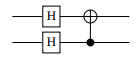
\includegraphics[width=0.9\linewidth]{quipper_1}
	\caption{The corresponding quantum circuit diagram}
\end{subfigure}
\small Code and diagram courtesy of \cite{quipper1}.
\end{figure}

The first line declares a function, \texttt{mycirc}, that takes two \texttt{Qubit}s as input and returns two \texttt{Qubit}s. Then, a Hadamard gate (a very common and useful gate in quantum computing) is applied to both \texttt{a} and \texttt{b}. Finally, a CNOT (controlled NOT) gate is applied, using \texttt{b} as a control.

Now that the gates are grouped into a single function, operations can be done on them as a whole. For example, \verb|with_controls| can be used to control an entire set of gates using a qubit or collection of qubits. Other higher-order operations include \verb|with_ancilla|, which provides ancillas\footnote{temporary scratch space in a quantum register} to a circuit; \verb|reverse_simple|, which accepts a quantum function and returns its inverse; \verb|decompose_generic|, which accepts a circuit, and returns a circuit with all gates from the original decomposed into a specified set of circuits.

By encapsulating these circuits within \texttt{Circ}, Quipper can separate the specification of a circuit from what is used for. Once a circuit is specified, operations can be called on the \texttt{Circ} monad containing it, such as rendering a representation of the circuit, simulating the circuit, or running it on a quantum computer (eventually).

With data types out of the way, we turn to Quipper's stages of execution. Because Quipper describes circuits, it has three distinct phases: compilation, circuit generation, and circuit execution. (This also occurs in hardware description languages such as Verilog.) The first two stages take place on a classical computer, while the third takes place on a quantum computer (or simulator). Compilation is fairly uninteresting; it is the same as standard Haskell compilation with linked libraries, turning source code into an executable meant for a classical computer. This leaves us to the exam the two run-times, the latter two stages.

After Quipper's code is compiled, it can be executed to generate the circuit. This stage takes circuit parameters, such as number of available qubits on the device and error thresholds, and outputs a representation of the quantum circuit. This representation could be an image to use as reference, a series of gates sent to a quantum computer, or some other format.

Finally, after the circuit is generated, it can be sent to a quantum computer for execution. The quantum computer can then accept inputs, such as classical bits or qubits from long-term storage should the device support it. The device will then process the circuit, however that may occur. Its outputs then mirror its input: classical bits and/or qubits for long-term storage.

Sometimes, however, the process is not so linear. Many quantum algorithms require alternating between circuit generation and circuit execution. The classical computer generates a circuit and sends it to the quantum computer; the measurement results are then fed back into the classical computer to generate another circuit, and so on. In Quipper, this is called \textit{dynamic lifting}. Quipper is designed to be general enough to support this and many other models of computation.

To wrap up our examination of Quipper, we will look at the features provided to developers. These are not strictly necessary to design quantum algorithms, but they make the process easier. These shall be separated into two categories for examination: features that make designing circuits easier and features that make understanding circuit diagrams easier.

First, we examine some common features of functional programming languages and how Quipper adapted them to work with quantum values. Quipper allows circuits to be built up with recursive functions, like other functional languages allow the final answer of a function to be built up through recursive calls. This is especially useful for functions that can take a list of \texttt{Qubit}s, such as the quantum Fourier transform. Quipper also implements the higher-order map function, which applies a quantum gate across every \texttt{Qubit} in a data structure.

Quipper also uses higher-order functions to manipulate circuits. Some such functions, such as \verb|reverse_simple| and \verb|decompose_generic|. In addition, it is possible to create user-defined manipulations and transformations. For example, suppose a programmer is implementing an algorithm for an architecture that doesn't support a specific gate; the programmer can create a transformation function to replace that gate with a gate (or set of gates) equivalent to it.

Next, consider the previously mentioned \verb|with_ancilla|. In quantum computing, an ancilla is analogous to a local variable; the value is necessary only for a block of code. Unlike local variables in a classical language, ancillas must be \textit{uncomputed} (that is, reset to an unentangled state) so as not to interfere with superpositions once out of scope. Quipper allows explicit scoping of ancillas and automatically allocates/deallocates them from quantum registers. At the end of an ancilla's scope, it can be \textit{assertively terminated}; that is, the programmer signals to the compiler that, at the end of its scope, the ancilla will be returned to its original state. This allows the compiler to make certain optimizations it could not otherwise, and allows it to reverse circuits containing ancillas. Uncomputing the ancillas is, however, the programmer's task; the compiler trusts that the program passes the assertion. Quipper accomplishes the use of ancillas by use of the \verb|with_ancilla|, which accepts a function (often a lambda\footnote{An anonymous function}) that takes a \texttt{Qubit} and generates a circuit. For use of multiple ancillas, Quipper provides \verb|with_ancilla_list|; this functions essentially the same, but it also accepts an integer to specify the number of ancillas required.

Quipper also allows for automatic generation of quantum oracles. Often, oracles are specified in a classical manner, but need to be applied to quantum data; Quipper provides the \verb|build_circuit| keyword and the \verb|classical_to_reversible| operator to solve this problem. By including \verb|build_circuit| before the definition of a function accepting and returning some number of \texttt{Bool}s, Quipper will generate a corresponding quantum function, accepting and returning some number of \texttt{Qubit}s. This function can be accessed by calling \verb|template_funcname|, where \texttt{funcname} is the name of the previously defined function. However, the programmer must provide quantum templates for any standard library functions used, if they are not one of the standard functions provided by Quipper. The functionality of \verb|build_circuit| is implemented using the Template Haskell extension for Haskell, which allows Quipper to modify a program's syntax tree at compile time.

However, the circuit generated by \verb|build_circuit| is not a standalone reversible circuit. Quipper will generate ancillas as necessary for the function, which are not automatically uncomputed. Fortunately, the \verb|classical_to_reversible| operator solves this; it converts a circuit $f :: a \to \texttt{Circ} b$ into its reversible counterpart, $f' :: (a, b) \to \texttt{Circ} (a, b)$. Assuming $f$ uses only reversible primitives, all ancillas will be properly uncomputed at the end of $f'$.

As for making circuit diagrams more readable, Quipper provides two noteworthy features: comments and hierarchical circuits. Comments are fairly self-explanatory; Quipper provides a function, \verb|comment_with_label|, that adds a comment to the circuit diagram and labels specified \texttt{Qubit}s. This is useful to keep track of where certain operations (e.g., quantum teleportation) take place, as well as which wire on the diagram represents which \texttt{Qubit}.

Hierarchical circuits help abstract away the details of repeated subcircuits. Often in quantum algorithms, a subcircuit (such as a quantum Fourier transform) is used many times. By turning it into a boxed subcircuit, using Quipper's \texttt{box} function, the subcircuit only has to be generated once. It is then represented as a labeled box, like any other gate, in the circuit diagram. To the side, Quipper renders the contents of the box. Because of this, developers looking at a diagram don't have to worry about exactly how a subcircuit works each time, nor do they have to focus on figuring out which subcircuit it is. Together, these two features can greatly simplify reading a diagram produced by Quipper.

In the end, Quipper is the most advanced quantum programming language embedded in Haskell. It adds natural quantum extensions to its functional host language, allowing the abstraction necessary for development of quantum programming languages. \cite{quipper1}

\subsection{LIQU$i|>$}
In 2015, Microsoft's QuArC\footnote{Quantum Architectures and Computation Group} released LIQ$Ui|>$\footnote{Language Integrated Quantum Operations}, a software architecture and toolset for quantum computing. It contained an extension to the high-level functional language F\#, allowing developers to express quantum circuits in a high-level language. It can also be used within any other language, such as C\#, that has the ability to interface with the LIQ$Ui|>$ library. Microsoft designed the software such that the results of compilation are independent of architecture. Like Quipper, it allows for a classical machine to provide control signals to a quantum device. However, unlike Quipper, it allows for non-physical operations, despite also being intended to be run on a real quantum machine.

LIQ$Ui|>$, like Quipper, draws upon preceding languages such as the quantum lambda calculus and the quantum IO Monad, while offering improvements. The developers described it as a reduction of the ideas drawn from those formal languages, turning them into a user-friendly and practical language. Many of the same improvements have been made in LIQ$Ui|>$ as in Quipper.

However, whereas Quipper was implemented in Haskell, Microsoft chose F\# as the host language for LIQ$Ui|>$. During design, they chose to shy away from Quipper's ideal of linear types. They argue that such types do not map well to a physical qubit, as qubit are mutable and may, in some cases, be non-destructively measured. They opt instead for a functional language with an isolated physical model. F\# was chosen for its support of both object-oriented and functional programming paradigms, as well as strong static typing. It also allows access to the program's syntax tree, much like Template Haskell does for Quipper. In addition, it cannot be overlooked that F\# is supported by Microsoft's Visual Studio development suite.

Now, we will examine the data types LIQ$Ui|>$ brings to F\#. Naturally, it contains \texttt{Bit} and \texttt{Qubit} types. \texttt{Bit} is a classical data type, capable of taking on values of \texttt{Zero, One,} and \texttt{Unknown}, where \texttt{Unknown} represents the value of a an unmeasured \texttt{Qubit}. A \texttt{Qubit} represents a single quantum value; after measurement, its \texttt{Bit} value will change from \texttt{Unknown} to either \texttt{Zero} or \texttt{One}.

To represent the state of the quantum machine, Microsoft designed the \texttt{Ket} type. It is the state vector representing all \texttt{Qubit}s in the system. Initially, it is a vector of size $n$, where $n$ is the number of \texttt{Qubit}s; however, as \texttt{Qubit}s become entangled, it can grow as large as $2^n$.

Both \texttt{Qubit}s and \texttt{Ket}s are implemented as opaque types; they can only interact with the rest of the program through a defined interface. Because of this, they can contain a (quantum) state, without detracting from their functional environment.

The \texttt{Gate} data type implements a quantum gate, allowing programmers to perform operations on \texttt{Ket}s. They can be as simple as a $2 \times 2$ unitary matrix\footnote{Knowing the actual definition of a unitary matrix is not important for this paper. There are a few properties that make this section easier to understand, though: unitary matrices are square, and you can invert them in order to reverse the gate.} operating on a single \texttt{Qubit}, or they can be more complex, such as the Controlled-NOT \texttt{Gate} or the Measurement \texttt{Gate}. Note that there are no \texttt{Gate}s truly built into the LIQ$Ui|>$; instead, they are included with the library for convenience. Because of this, all gates may be extended as desired by the user.

Since each \texttt{Gate} is just a data structure, they have a corresponding F\# function, known as an \texttt{Operation}, that carries out the definition of the \texttt{Gate} it contains. This separation allows each \texttt{Operation} to be called in multiple modes (Run, Circuit, and Gate). Once an \texttt{Operation} is created, it is as natural to call it as any other function in F\#. For example, to run the Hadamard gate (Denoted \texttt{H}) on a \texttt{Qubit q}, one can simply type \texttt{H q}.

A sequence of \texttt{Operation}s can then be wrapped in a data structure called a \texttt{Circuit}. This allows them to be analyzed, modified or optimized, rendered, or simply run. LIQ$Ui|>$'s optimization will be touched on later. As with Quipper, we will now create a simple function in LIQ$Ui|>$, representing the same circuit.


\begin{figure}
	\label{fig:liquid_1}
	\caption{A simple example of functions in LIQ$Ui|>$}
	\begin{subfigure}{0.7\textwidth}
		\begin{lstlisting}[language=Haskell]
let mycirc()    =
	let ops(qs:Qubits)    =
		let a,b    = qs.[0],qs.[1]
		H qs
		CNOT[b;a]
		M >< qs
	
	let ket    = Ket(2)
	let qs    = ket.Qubits
	
	let circ    = Circuit.Compile ops qs
	circ.Run qs
		\end{lstlisting}
	\end{subfigure}
	\begin{subfigure}{0.3\textwidth}
		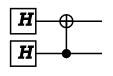
\includegraphics[width=0.9\linewidth]{liquid_1}
		\caption{The corresponding quantum circuit diagram generated by LIQ$Ui|>$}
	\end{subfigure}
\end{figure}

Similar to Quipper, these gates can now be manipulated as a whole. For example, one could call \texttt{circ.Reverse()} to reverse the circuit; \texttt{AddControl} can be used to turn them into controlled gates; and the gates can be 'grown', from a sequence of unitary gates to a single, larger gate, greatly shortening runtime.

LIQ$Ui|>$ also works with three separate stages of execution: compilation, circuit generation, and circuit execution. Again, compilation is not a very interesting stage, as it is simply standard F\# compilation. During circuit generation, the language optimizes various parts of the circuit: collapsing sequential unitary gates into a single unitary gate, replacement of gates unavailable to the chosen architecture, optimizing the depth of the circuit, and more. After that, LIQ$Ui|>$ outputs a data structure representing the circuit, capable of being fed to another system, and/or generates a graphical representation of the circuit.

Circuit execution is very similar to Quipper: it is designed to be sent to a quantum computer. However, Microsoft included a variety of useful features for debugging quantum algorithms on a simulator. Included with LIQ$Ui|>$ is a debugger, allowing programmers to examine the usually opaque state of a simulated quantum machine without collapsing superposition. It also allows injection of noise in order to more realistically test a circuit. Finally, like Quipper, it allows interleaving of quantum computation and classical control.

Finally, we end our examination of LIQ$Ui|>$ with an inspection of features it provides to ease reading and writing of circuits. Again, as with Quipper, it allows gates to be decomposed into simpler gates, and circuits to be easily reversed. LIQ$Ui|>$ does not provide as easy management of ancillas as Quipper; the user must directly allocate them. It does, however, provide a \texttt{Reset} operation to set \texttt{Qubit}s to $\ket{0}$ or $\ket{1}$. Like Quipper, it allows user-defined circuit manipulations and transformations, as well as support for exporting to a certain architecture. Although LIQ$Ui|>$ does allow for the defining of quantum oracles, it does not provide an operation to automatically generate one from a classical oracle.

As for making reading of diagrams easier, LIQ$Ui|>$ provides the same functionality as Quipper. The language allows programmers to build up circuits from the low-level---singular gates---to higher levels of abstraction, representing entire subciruits with a single gate. LIQ$Ui|>$ calls this feature gate wrapping, and implements it using \texttt{WrapOp}. This can simplify circuit diagrams when they are generated. It also allows for parts of a circuit to be labeled, making understanding the circuits easier.

LIQ$Ui|>$ is an excellent functional programming language and quantum development suite. It allows programmers to build quantum algorithms from the ground up, manipulating them at low and high level, and then simulate and debug their algorithms. Given that it is created by Microsoft, its development will likely continue, giving it a lot more promise than independently developed programming languages. \cite{liquid1}

\section{Conclusion}
Quantum computation is still in its infancy, and it may be some time until a quantum machine advanced enough to run nontrivial algorithms is available. However, the development of quantum programming languages is still promising and will continue to advance as more research is done into quantum computation. The dramatic shift in thinking necessary to program quantum algorithms instead of classical algorithms will be difficult for many programmers, but ultimately the development of quantum programming languages will make the transition easier.

\section{References}
\printbibliography

\section{Appendix: Implementations of Grover's Algorithm}
\subsection{Quipper}
\begin{lstlisting}[language=Haskell]
import Quipper

-- declare Oracle data type
data Oracle = Oracle {
	qubit_num :: Int,
	function :: ([Qubit], Qubit) -> Circ ([Qubit], Qubit)
}

-- declare phase_inversion function
phase_inversion::(([Qubit],Qubit)->Circ([Qubit],Qubit))->([Qubit],Qubit)-> Circ([Qubit],Qubit)
phase_inversion oracle (top_qubits, bottom_qubit) = do
	comment "start phase inversion"
	-- call oracle
	oracle (top_qubits, bottom_qubit)
	comment "end phase inversion"
	return (top_qubits, bottom_qubit)

-- declare inversion_about_mean function
inversion_about_mean :: ([Qubit], Qubit) -> Circ ([Qubit], Qubit)
inversion_about_mean (top_qubits, bottom_qubit) = do
	comment "start inversion about mean"
	-- apply X gate at top qubit
	mapUnary gate_X top_qubits
	-- separate target and control qubits
	let pos = (length top_qubits) - 1
	let target_qubit = top_qubits !! pos
	let controlled_qubit = take pos top_qubits
	-- apply hadamard at target_qubit
	hadamard_at target_qubit
	-- apply qnot gate at target qubit
	qnot_at target_qubit ‘controlled‘ controlled_qubit
	-- apply hadamard again at top
	hadamard_at target_qubit
	-- apply X gate at bottom
	mapUnary gate_X top_qubits
	comment "end inversion about mean"
	return (top_qubits, bottom_qubit)
	
-- declare grover_search_circuit function
grover_search_circuit :: Oracle -> Circ ([Bit])
grover_search_circuit oracle = do
	comment "Grover Search algorithm"
	-- set the value of n
	let n = toEnum (qubit_num oracle) :: Float
	-- set the index number to iterate sqrt(2^n) times
	let index = (floor (sqrt (2**n))) :: Int
	-- create the ancillaes
	top <- qinit (replicate (qubit_num oracle) False)
	bottom <- qinit True
	label (top, bottom) ("|0>","|1>")
	-- apply hadamard gate at string
	mapUnary hadamard top
	hadamard_at bottom
	-- start to iterate
	for 1 (index) 1 $ \i -> do
		comment "start grover iteration"
		-- call phase inversion
		(top, bottom) <- phase_inversion (function oracle) (top, bottom)
		-- call inversion about mean
		(top, bottom) <- inversion_about_mean (top, bottom)
		comment "after grover iteration"
	endfor
	-- measure qubit string and return result
	hadamard_at bottom
	(top, bottom) <- measure (top, bottom)
	cdiscard bottom
	return (top)
	
-- main function
main = print_generic Preview (grover_search_circuit empty_oracle)
where
	-- declare empty_oracle’s data type
	empty_oracle :: Oracle
	empty_oracle = Oracle {
		-- set the length of qubit string
		qubit_num = 4,
		function = empty_oracle_function
	}
	-- initialize empty_oracle’s function f(x)
	empty_oracle_function:: ([Qubit],Qubit) -> Circ ([Qubit],Qubit)
	20
	empty_oracle_function (ins,out) = named_gate "Oracle" (ins,out)
\end{lstlisting}
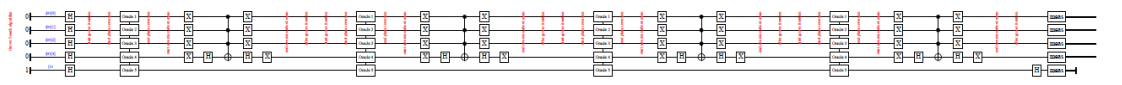
\includegraphics[width=0.9\linewidth]{quipper_grover}

{\small Code and diagram courtesy of \cite{quipper2}.}

\subsection{LiQ$Ui|>$}
\begin{lstlisting}[language=Fsharp]
// define the quantum oracle
// will negate phase if all qubits are |1>
let oracle (qs:Qubits) =
	let gate (qs:Qubits)    =
		let parent  = !< Z !!qs.[qs.Length-1]
		parent.AddControl(qs.Length-1)
	(gate qs).Run qs

let grover_circ (qs:Qubits) =
	// apply Z to the last qubit if all other bits are 1
	let CFZ = (!< Z qs).AddControl(qs.Length-1)

	// set each qubit to 1 then apply a Hadamard gate
	// in order to achieve a superposition
	X >< qs
	H >< qs
	
	// apply Grover's Diffusion sqrt(2^n) times
	for i in 1..(int (sqrt (2.0**(float qs.Length)))) do
		oracle qs
		H >< qs
		CFZ.Run qs
		H >< qs
	M >< qs
\end{lstlisting}
{\small Code implemented by Isaac Speed, using LIQ$Ui|>$ \cite{liquid1}}
\end{document}
